\chapter{Le cloud computing}
\begin{onehalfspace}

\initial{L} e but de ce chapitre est d'exposer le travail fait au niveau de la documentation. Ce chapitre est très riche par des concepts incontournables à la suite de ce rapport. En effet, nous allons commencer par expliquer ce que signifie le cloud concrètement. Ensuite nous présenterons les types de cloud les plus classiques, à savoir IaaS, PaaS et SaaS. Enfin, les notions machines virtuelles et conteneurs seront présentées avec une comparaison détaillée des deux.


\newpage


\section{Le Cloud Computing}

\subsection{Définition}

Le \textbf{Cloud Computing} est l'exploitation de la puissance de calcul ou de stockage de serveurs informatiques distants par l'intermédiaire du réseau internet. Ces serveurs sont loués à la demande selon des critères technique (Bande passante, puissance, etc.). Le cloud computing se caractérise par sa grande souplesse. En effet, il est déstiné aux utilisateurs de tous les niveaux de compétences.

Le cloud est rendu possible grâce à la virtualisation, l'ubiquité des réseaux à grande vitesse, les capacités des navigateurs d'aujourd'hui et l'évolution des piles de développement Web. Avec ces choses en place, il devient moins nécessaire de posséder votre propre infrastructure, ou même de posséder votre propre logiciel. Vous pouvez obtenir ce que vous avez besoin à partir du Cloud, tant que vous en avez besoin.


\subsection{Caractéristiques}

En termes clairs, le Cloud donne la capacité pour les utilisateurs finaux d'utiliser des pièces de ressources. Ces ressources doivent être acquises rapidement et facilement. NIST définit plusieurs caractéristiques qu'il juge essentiel pour qu'un service soit considéré comme «Cloud». Ces caractéristiques comprennent:

\begin{itemize}

\item Service à la demande. La capacité pour un utilisateur final de s' inscrire et recevoir des services sans les longs délais qui ont caractérisé l'informatique traditionnelle;

\item Accessible au réseau large. La Capacité d'accéder au service via les plates-formes standard (bureau, ordinateur portable, mobiles, etc.);

\item La mise en commun des ressources. Les fournisseurs servent plusieurs clients ou «locataires» avec des services provisoires et scalables. Ces services peuvent être ajustés pour répondre aux besoins de chaque client, sans aucune modification apparente pour l'utilisateur;

\item Rapide élasticité. La capacité des ressources doit évoluer pour faire face aux pics de la demande;

\item Service mesuré. La facturation est mesuré et livré


\end{itemize}

Sans ces caractéristiques, l'informatique en nuage n'appore rien par rapport à l'informatique traditionnelle. Une solution Cloud doit démontrer ces caractéristiques et notre projet ne doit pas échapper à cette règle. Dans ce qui suit, nous détaillerons les types classiques du cloud.

\subsection{Les types de Cloud}

Le Cloud Computing est un large terme qui décrit une large collection de services. Dans ce rapport, nous allons expliquer les différents types de services de Cloud communément appelé Software as a Service (SaaS),  Platform as a Service (PaaS) et Infrastructure as a Service (IaaS) et décrirent plus en détails ceux qui touchent à notre sujet.

\begin{figure}[H]
\centering
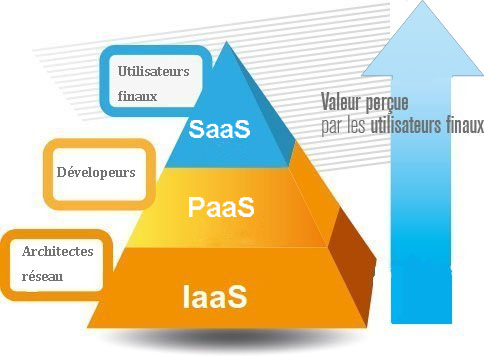
\includegraphics [scale=0.7]{chapitre2/assets/pyramide.jpg}
\caption{Pyramide des services Cloud}
\end{figure}

\subsubsection*{Software as a Service}

La meilleure façon de comprendre ces services est de commencer avec le SaaS, la couche la plus abstraite et celui qu'on utilise peut-être déjà aujourd'hui, même à un niveau personnel. Un exemple simple de SaaS est un service de messagerie en ligne, comme Gmail. Lorsque l'on utilise Gmail, vous n'êtes pas hébergez votre propre serveur de messagerie. C'est Google qui l'héberge, et on est tout simplement entrain d'y accéder via un navigateur comme un client.

SaaS est vraiment orienté vers les utilisateurs finaux de l'entreprise et ne nécéssite pas beaucoup de compétences pour l'utiliser. Le fournisseur décide sur le nombre de ressources à consacrer à l'utilisation de l'application. Le fournisseur décide sur les serveurs, les machines virtuelles, l'équipement de réseau, tout. Enfin, il suffit de pointer le navigateur à l'application.

\subsubsection*{Infrastructure as a Service}

IaaS est à l'autre bout du pyramide du Cloud. Lorsque l'on souhaite garder le contrôle de l'environnement logiciel, mais on veut pas maintenir aucun équipements; Lorsque l'on veut pas acheter des serveurs et de les mettre dans une pièce à température contrôlée ou rien de tout cela; On va chez un fournisseur IaaS et demander tout simplement une machine virtuelle.

L'on peut mettre n'importe quel logiciel que l'on souhaite au-dessus d'IaaS. Sur l'arrière, le fournisseur obtient vous de stockage ou d'autres ressources que l'on a besoin. Ceci est rendu plus facile avec les technologies de virtualisation, qui séparent les ressources physiques de la machine virtuelle qui éxécute le logiciel. IaaS est disponible sur Amazon EC2, GCE de Google et bien d'autres.

L'infrastructure en tant que service ou l'IaaS ne touche pas directement à notre sujet. Du coup, il ne sera mentionné que rarement par la suite.

\subsubsection*{Platform as a Service}

PaaS se situe quelque part entre IaaS et SaaS. Il est pas un produit fini, comme SaaS, encore moins une simple ressource virtuelle vierge, comme IaaS. PaaS est destiné pour les développeurs, il leur donne des outils et des interfaces de haut niveau pour y développer dessus. Par exemple, Windows Azure de Microsoft vous donne des outils pour développer des applications mobiles, des applications sociales, sites Web, jeux et plus encore. Vous construisez ces choses, mais vous utilisez les API et les outils pour les accrocher dans l'environnement Azure et de les exécuter là.


\begin{figure}[H]
\centering
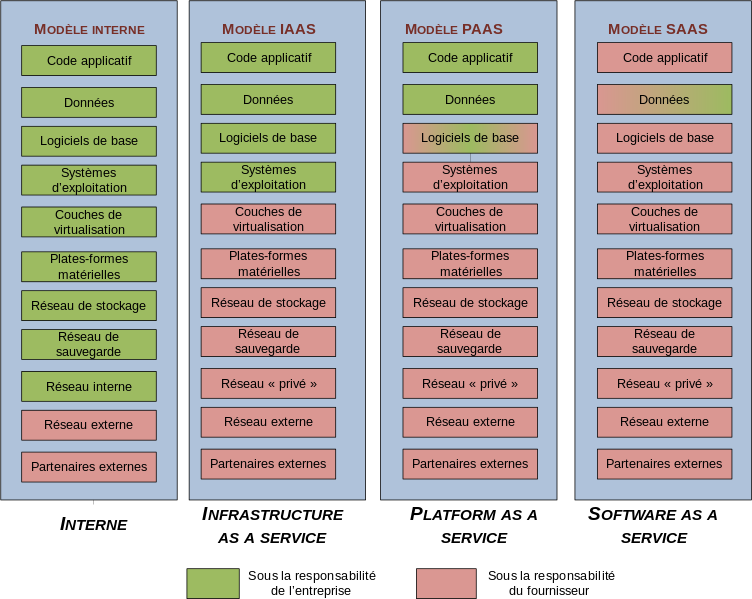
\includegraphics [scale=0.5]{chapitre2/assets/cloud-vs.png}
\caption{L'éxternalisation de l'informatique en Cloud}
\end{figure}


\section{Virtualisation ou containérisation}

\subsection{Virtualisation}

Avec des racines profondément ancrées dans l'informatique, la virtualisation sert à partitionner un seul serveur physique en plusieurs machines virtuelles, comme un espace de stockage ou un réseau, en plusieurs ressources virtuelles. Elle permet une consolidation de serveurs avec une grande souplesse d'utilisation. Dans le contexte de l'informatique en nuage, la virtualisation est importante pour la mise en service et le retrait rapide de serveurs. Ceci étant dit, la scalabilité est la principale caractéristique du Cloud moderne, faute de cela, on ne peut en parler. Ainsi la virtualisation a permis de créer des machines virtuelle, les faire monter en charge à la demande, faire de la migration à chaud, etc. Un logiciel de virtualisation du Cloud présente également une perspective dynamique et une vue unifiée de l'utilisation et de l'efficacité des ressources, cela afin d'assurer le fonctionnement des services du Cloud. La virtualisation est une technologie permettant d'arriver à une utilisation rentable des serveurs tout en prenant en charge la séparation entre de multiples locataires d'un matériel physique.

Il existe plusieurs solutions de virtualisation, l'on peut citer à titre informatif:

\begin{itemize}
\item VMware, Cette solution, séduisante, pose certains problèmes. En effet, il propose des outils propriétaires et incompatible avec le noyau Linux;
\item Xen est un hyperviseur libre de machines virtuelles, il est considéré comme un outil de virtualisation des plus performants;
\item KVM, Kernel-based Virtual Machine est devenue rapidement la solution de virtualisation de référence pour Linux. Elle est basée sur les architectures Intel ou les architectures AMD;
\item QEMU, est un émulateur machine générique. C'est une solution de virtualisation à utiliser si le processeur de système hôte ne possède pas d'extension matérielle spécifique à la virtualisation.

\end{itemize}

\subsection{Containérisation}

Noyau Linux permet de lancer plusieurs instances isolées de l'espace utilisateur. Un conteneur est un environnement isolé où un ou plusieurs processus peuvent être exécutés. Les conteneurs se concentrent sur l'isolation des processus au lieu d'émuler une machine physique complet.

Historiquement, chroot dans le noyau Linux a fourni un certain niveau d'isolation en fournissant un environnement pour créer et héberger une copie virtualisée d'un logiciel, et ceci depuis le début des années 80. Mais le terme «conteneurs» n'est pas venu jusque vers la fin de l'année 2006. Il a été renommé «Control Groups» (cgroups) pour éviter toute confusion causée par de multiples significations du terme «conteneurs» dans le noyau Linux. «Control Groups est une fonctionnalité du noyau linux qui est disponible depuis la version v2.6.24, elle limite et isole l'utilisation des ressources d'un ensemble de processus. Par la suite, l'isolation de l'espace de noms a été ajouté.

Cela a conduit à l'évolution de Linux Containers (LXC), un environnement de virtualisation au niveau du système d'exploitation qui est construit sur les fonctionnalités du noyau Linux mentionnés plus haut, comme chroot, cgroupes, l'isolation de l'espace de noms, etc.

\paragraph{Cgroups}

\begin{itemize}
\item Isolation de l'usage des ressources (CPU, mémoire, E/S, etc.);
\item Limitation des ressources: un groupe peut être configuré pour ne pas dépasser une certaine limite de la mémoire;
\item Priorité: certains groupes peuvent obtenir une plus grande part de CPU ou de débit E/S disque;
\item Mesure de l'usage des ressources;
\item Contrôle: le gel des groupes ou des points de reprise et le redémarrage.
\end{itemize}

\paragraph{Namespaces}
\begin{itemize}
\item Partionnement des structures de kernel pour créer des environnements virtuels
\item Des espaces de noms différents

\begin{itemize}
\item pid (processus)
\item net (interfaces réseaux, routage, ...)
\item ipc (communication inter-processus)
\item mnt (points de montage, système de fichiers)
\item uts (Nom de hôte)
\item user (UIDs)
\end{itemize}

\end{itemize}


\paragraph{}
Contrairement à la virtualisation, la liste des solutions de containérisations n'est pas aussi longue. La plupart d'eux se basent sur ou convergent vers cgroups et namespaces. L'on cite:

\begin{itemize}
\item LXC, Linux containers, combine cgroups et namespace pour fournir un environnement isolé pour les applications;
\item OpenVZ permet de créer multiples conteneurs pour Linux. Dorénavant, tous les efforts des développeurs d'OpenVZ vont aller dans le sens de fusionner les fonctionnalités d'OpenVZ avec LXC;
\item lmctfy, Let Me Contain That For You, est une solution open source de containérisation de Google qui est basé sur cgroups. Le futur de lmctfy est flou vu que Google avait commencé à migrer les concepts de lmctfy vers Docker;
\item Docker, ce n'est pas une autre solution, mais il est basé sur LXC et fournit une couche de haut niveau accessible pour l'utilsateur;

\end{itemize}

\subsection{Etude comparative}

Le choix de la solution a été proposé fortement par la société. On a opté pour une solution de containérisation (Docker) dans la mesure où un benchmark prouve son efficacité et sa légèreté.





\section{Docker}

\end{onehalfspace}